%&tex
% !TEX program = xelatex
% !TeX TS-program = xelatex
% !BIB TS-program = biber
% !TeX encoding = UTF-8
% !TeX spellcheck = en_US
% !TeX root = ./thesis.tex
% !TeX document-id = {4b2b7ac1-93c5-4ea7-94ea-3424b3592d6f}

%% Version: 0.6 (03.01.2019)

%% Choose language: english or german
%% Choose Thesis type: seminar, bachelor, master, phd, techreport
%% Use 'declaration' parameter if you want to generate declaration page
%% Use 'final' to disable Todo-notes from final version without deleting each one of them
\documentclass[english,seminar]{KITthesis}

%% ---------------------------------
%% | Information about the thesis  |
%% ---------------------------------
%% Version: 0.8 (12.02.2019)

%% My_document_info.tex
%% Copyright 2020 KIT, IAR-IPR (Denis Štogl)
%% Mail: denis.stogl@kit.edu
%
% This work may be distributed and/or modified under the
% conditions of the LaTeX Project Public License, either version 1.3
% of this license or (at your option) any later version.
% The latest version of this license is in
%   http://www.latex-project.org/lppl.txt
% and version 1.3 or later is part of all distributions of LaTeX
% version 2005/12/01 or later.
%
% This work has the LPPL maintenance status `maintained'.
%
% The Current Maintainer of this work is M. Y. Name.
%
% This work consists of the files pig.dtx and pig.ins
% and the derived file thesis.tex.


\title{Automated Programming of PLCs}
\titleotherlanguage{Automatische Programmierung von PLCs}

\author{David Oberacker}
\address{Jarnyweg 13}
\city{76351 Linkenheim-Hochstetten}
\email{david.oberacker@student.kit.edu}

\keywords{Keywords, of, my, Thesis, Keywords, of, my, Thesis, Keywords, of, my, Thesis, Keywords, of, my, Thesis, Keywords, of, my, Thesis, Keywords, of, my, Thesis, Keywords, of, my, Thesis}
\keywordsotherlanguge{Die, Stichw\"orter, f\"ur, meine, Arbeit, Die, Stichw\"orter, f\"ur, meine, Arbeit, Die, Stichw\"orter, f\"ur, meine, Arbeit, Die, Stichw\"orter, f\"ur, meine, Arbeit, Die, Stichw\"orter, f\"ur, meine, Arbeit}

%% Study program or a seminar/subject
\studyprogram{Intelligente Industrieroboter}

%% IMPORTANT: Seminar only: If not "Seminar Intelligente Industrieroboter" uncomment this
% \nogrouplogo

%% Name of your institute (Default: IAR-IPR)
% \institute{Test}
%% Name of your faculty (Default: KIT-Fakultät für Informatik
% \KITfaculty{This is my Faculty}
%% Address of your institute (Default: Engler-Bunte-Ring 8)
% \instituteaddress{}
% %% Insitute City (Default: 76131 Karlsruhe)
% \institutecity{}

\reviewerone{Prof. Dr.-Ing. Torsten Kröger}
\reviewertwo{Prof. Dr.-Ing. habil. Björn Hein}
%
% %% The advisors are PhDs or Postdocs
\advisorone{Dr.-Ing. Christoph Ledermann}
% %% The second advisor can be omitted
%\advisortwo{M.Sc. D}
%
% %% Please enter the start end end time of your thesis (for techreport not needed)
\editingtime{24. April 2020}{09. Juli 2020}

%% --------------------------------
%% | Settings for word separation |
%% --------------------------------
% Help for separation:
% In german package the following hints are additionally available:
% "- = Additional separation
% "| = Suppress ligation and possible separation (e.g. Schaf"|fell)
% "~ = Hyphenation without separation (e.g. bergauf und "~ab)
% "= = Hyphenation with separation before and after
% "" = Separation without a hyphenation (e.g. und/""oder)

% Describe separation hints here:
\hyphenation{
% Pro-to-koll-in-stan-zen
% Ma-na-ge-ment  Netz-werk-ele-men-ten
% Netz-werk Netz-werk-re-ser-vie-rung
% Netz-werk-adap-ter Fein-ju-stier-ung
% Da-ten-strom-spe-zi-fi-ka-tion Pa-ket-rumpf
% Kon-troll-in-stanz
}

%%
%% --------------------
%% |   Bibliography   |
%% --------------------
\newcommand{\mybibliographyfiles}{Bibliography/my_thesis_bibliography}


%% --------------------
%% |     Acronyms     |
%% --------------------
\newacronym{acn:ipr}{IAR-IPR}{Institute for Anthropomatics and Robotics - Intelligent Process Control and Robotics}
\newacronym[plural=PLC's,firstplural=\glspl{gls:plc} (PLC's)]{acn:plc}{PLC}{\gls{gls:plc}}

\newacronym{acn:ST}{ST}{Structured Text}
\newacronym{acn:IL}{IL}{Instruction List}

\newacronym{acn:LD}{LD}{Ladder Diagram}
\newacronym{acn:FBD}{FBD}{Function Block Diagram }

\newacronym{acn:SFC}{SFC}{Sequential Function Chart}

\newacronym{acn:ml}{ML}{Machine Learning}

%% --------------------
%% |     Glossary     |
%% --------------------
\newglossaryentry{gls:robot}
{
    name=robot,
    description={The robot developed in this work.}
}

\newglossaryentry{gls:plc}{
	name={Programmable Logic Controller},
	plural={Programmable Logic Controllers},
	description={
		A programmable logic controller (PLC) or programmable controller is an industrial digital computer which has been ruggedized and adapted for the control of manufacturing processes, such as assembly lines, or robotic devices, or any activity that requires high reliability, ease of programming and process fault diagnosis.~\cite{Wiki:Plc}
	}
}


%% ------------------------
%% |    Including files   |
%% ------------------------
% Only files listed here will be included!
% Userful command for partially translating the document (for bug-fixing e.g.)
\includeonly{%
	Content/0-Declaration,
	%Content/0-Abstract_EN,
	%Content/0-Abstract_DE,
	Content/1-Introduction,
	Content/2-PLC-General,
	Content/3-C-Based-Programming,
	Content/4-Formal-Methods,
	Content/5-Risks,
	Content/8-Conclusion,
%	Content/11-Appendix,
}

\settitle
\addbibresource{Bibliography/my_thesis_bibliography.bib}

%%%%%%%%%%%%%%%%%%%%%%%%%%%%%%%%%
%% Here, main documents begins %%
%%%%%%%%%%%%%%%%%%%%%%%%%%%%%%%%%
\begin{document}
    
    \selectlanguage{UKenglish}
	
	%% Uncomment this to use only first authors name in bibliography
	% \bstctlcite{BSTcontrol}
	
	%% Set PDF metadata
	\setpdf
	
	%% Title Page
	\includetitle
	
	% TODO: Remove this from final version
	\includelistoftodos
	
	\includedeclaration
	
	%\includeacknowledgments
	
	%% ----------------
	%% |   Abstract   |
	%% ----------------
	%% An abstract both in English
	%% and German is mandatory.
	%%
	%% The text is included from the following files:
	%% - Content/0-Abstract_EN
	%% - Content/0-Abstract_DE
	%\includeabstract
	
	%% ------------------------
	%% |   Table of Contents  |
	%% ------------------------
	\inculdetableofcontents
	
	\makenomenclature
	
	%% -----------------
	%% |   Main part   |
	%% -----------------
	\setmainpart
	
	%&tex
% !TEX program = xelatex
% !TeX TS-program = xelatex
% !BIB TS-program = biber
% !TeX encoding = UTF-8
% !TeX spellcheck = en_US
% !TeX root = ../thesis.tex

%% ==============================
\section{Introduction}
\label{sec:Introduction}
%% ==============================

\glspl{acn:plc} are a staple of industrial automation since the early 1970's.
They are used to automate and control all kinds of industrial tasks, from manufacturing equipment to fluid control systems~\cite{Erickson:1996aa}.
They can easily be maintained and extended due to their simplicity and modularity.
This allows for long runtime while being flexible enough to adapt to changes in the manufacturing process.

In contrast to the modularity in hardware, the software running on a~\gls{acn:plc} is more static.
The common way of programming a PLC is with on of the five languages defined in the \textit{IEC 61131-3} standard~\cite{Plcopen:61131-3}.
This standard defines two textual languages (\gls{acn:IL} and~\gls{acn:ST}), two graphical languages (\gls{acn:LD} and~\gls{acn:FBD}) and one hybrid language (\gls{acn:SFC}).
The focus of the standard languages is, to allow electrical and automation engineers to program the~\gls{acn:plc} in way that is close to common electrical relays.
Reasoning behind this is to keep the~\gls{acn:plc} as close to the previously used non programmable relays as possible.
Therefore the graphical languages are composing low level logical operations to generate outputs.
The textual languages allow for a more high level view on the operations while still operating close to the basic logical operations.

This makes building more complex applications on a~\gls{acn:plc} harder and reduces the flexibility of the systems to adapt from a software side.
When~\glspl{acn:plc} and the corresponding languages were designed this level of flexibility was sufficient, but with the rise of Industry 4.0, more flexible and integrated automation solutions are more important than ever.
For example the current development in~\gls{acn:ml} for industrial applications makes, adapting automation systems to allow for the quick access to sensor data or use the data provided by a~\gls{acn:ml} system, a requirement.
This makes faster development without the expense of formal correctness a high priority for automation solutions.
The developers of these automation solutions need to adapt to changes quicker and more often, with the changes requiring larger, more complex solutions.
In common high-level languages, like C/C++ or Python, extensive libraries and high-level abstractions can reduce the time it takes to create such a piece of software, whereas with the common~\gls{acn:plc} languages this isn't the case.
Due to the static and low-level approach to~\gls{acn:plc} programming other ways have to be found to allow for quicker and more integrated development of solutions.

\paragraph{Objective}
Therefore this seminar work investigates different approaches to automated~\gls{acn:plc} programming from high level abstractions.
I investigate the state-of-the-art on different approaches to automated~\gls{acn:plc} programming.
For this I look at different transformations and the related risks for usage in real world scenarios.

\paragraph{Method}
There are several different approaches from the past decades to this question.
One possible way of reducing programming time, is to allow C or C++ code to run on the~\gls{acn:plc}, allowing to make use of its high level abstractions.
Another possibility is to use a model or a formal description of the systems behavior to generate a program realizing it on a~\gls{acn:plc}.
Both approaches have found usage in recent years, as they have inherent strengths and weaknesses in the context of automation.
For this reason both I investigate both approaches to this problem.
This allows me to give a good overview of the current state-of-the-art for modern~\gls{acn:plc} program development.

\paragraph{Outline}
The following work will be structured as follows: 
Section~\ref{sec:plc} outlines the basics of~\glspl{acn:plc} and the IEC 61131-3 languages. 
Section~\ref{sec:c_methods} discusses methods to program a~\gls{acn:plc} with the high level languages C and C++.
Section~\ref{sec:formal_methods} investigates the state-of-the art of formal model based program generation and compares the different approaches.
As automated program generation in a often safety critical environment is risk, section~\ref{sec:risks} analyzes the risks of the presented solutions.
Finally, section~\ref{sec:conclusion} gives an overview of the found approaches and risks and summarizes the findings.
	%&tex
% !TEX program = xelatex
% !TeX TS-program = xelatex
% !BIB TS-program = biber
% !TeX encoding = UTF-8
% !TeX spellcheck = en_US
% !TeX root = ../thesis.tex
%% ==============================
\section{Programmable Logic Controllers}
\label{sec:plc}
%% ==============================

 
\begin{figure}
    \centering
    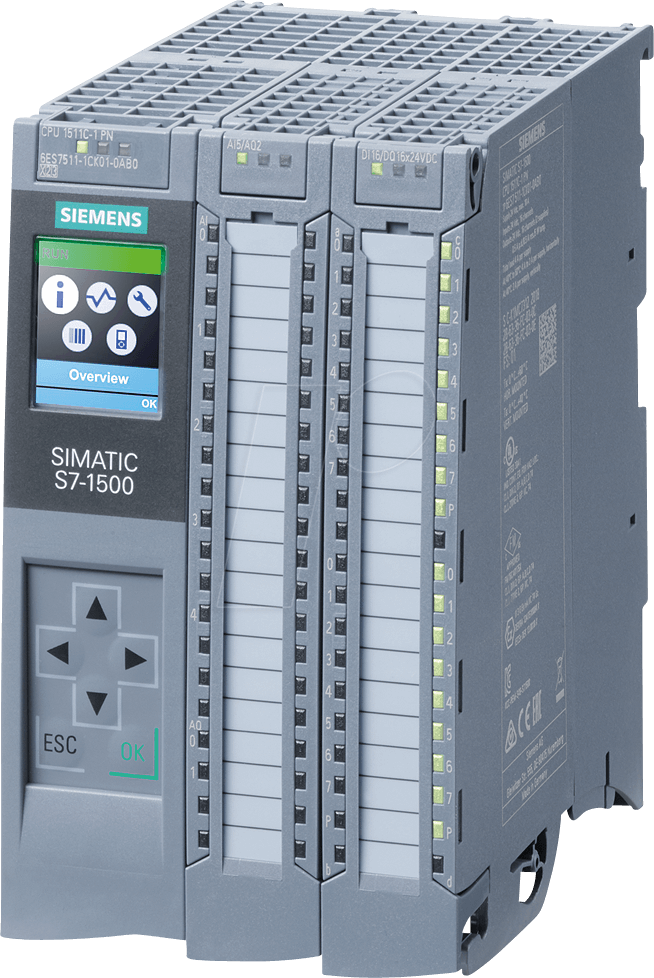
\includegraphics[width=0.5\textwidth]{Figures/simatic_s7-1500.png}
    \caption[Siemens SIMATIC S7-1500]{Siemens SIMATIC S7-1500~\acrshort{acn:plc}~\cite{Reichelt:2020}}
    \label{fig:simatic_s7}
\end{figure}

This section explains the basics of~\glspl{acn:plc} and their programming model.
They are a staple of industrial automation since the mid to late 1970's.
Major manufactures include Siemens, Rockwell Automation (Allen Bradley), Schneider Electric, Mitsubishi Electric, Omron, ABB, and General Electric~\cite{Businesswire:2016}.
Figure~\ref{fig:simatic_s7} shows an example of a modern Siemens mid-range~\acrshort{acn:plc} with an attached power supply and a I/O module is shown in figure.

\subsection{General}

\begin{figure}
    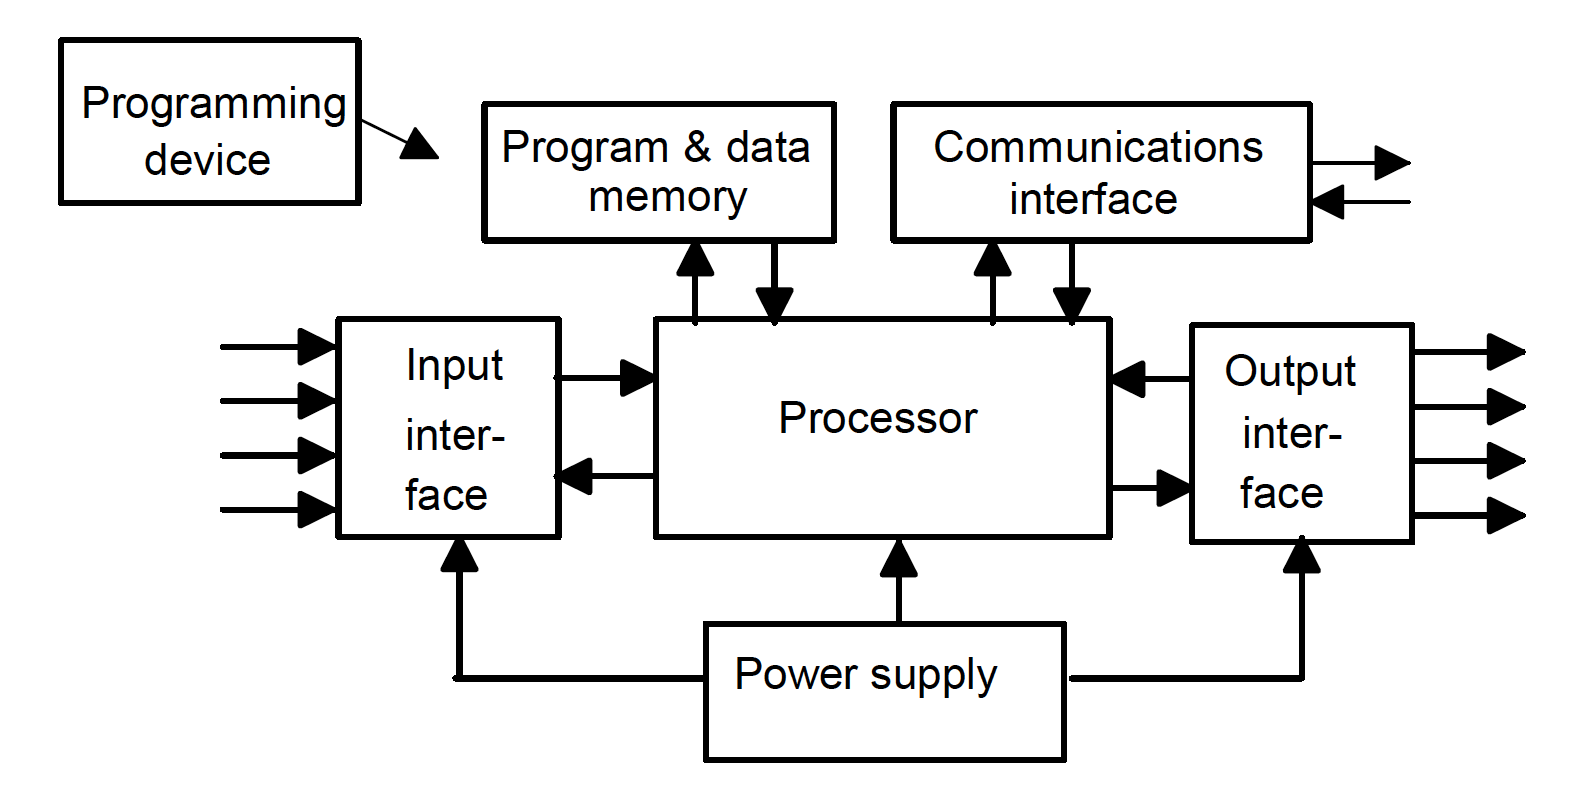
\includegraphics[width=\textwidth]{Figures/PLC_Architecture.png}
    \caption[PLC Architecture]{
       PLC Architecture~\cite[p.~4]{BOLTON200653}.
    The input and output interfaces are either digital or analog electrical signals.
    Memories are controlled by the OS on the PLC and are programmed with an external programming device.
    Additionally, PLC have a communications interface that allows it to communicate with other controllers or devices.}
    \label{fig:plc_architecture}
\end{figure}

A~\acrfull{acn:plc} is a controller that can be programmed via simple instructions to allow the easy processing of inputs and outputs~\cite[p.~4]{BOLTON200653}.
Figure~\ref{fig:plc_architecture} shows the basic components of a~\acrshort{acn:plc}.
\acrshort{acn:plc}s consist of input and output interfaces as well as a CPU that executes the current program on the inputs.
The program memory allows to change the programming of  the~\acrshort{acn:plc} without adapting any hardware components.
Additionally, the data memory can be used to persist data for creating stateful programs.
Lastly~\acrshort{acn:plc} contain a communications interface that allows the communication with other controllers or a supervisor software.
This can for example also be used to send sensor data to a central database or implement a self-management system.

A major advantage of~\acrshort{acn:plc} is that they allow for a modular design~\cite[p.~12]{BOLTON200653}, as seen with the Siemens~\acrshort{acn:plc} in figure~\ref{fig:simatic_s7}.
They are commonly assembled in a rack which allow to combine multiple modules to create a flexible configuration.
Additional hardware components, such as memory, processors, communication or I/O modules can be added with minimal effort.
This allows for standardized yet individually configurable hardware setups.
Many vendors also provide non modular single-box solutions.

Another difference between a~\acrshort{acn:plc}s and a regular micro-controller is the execution semantic of a program.
\acrshort{acn:plc} programs are executed in repeating cycles.
Each cycle consists of three distinct phases: reading of input values into the~\acrshort{acn:ram}, execution of the program and the writing of the output variables from the~\acrshort{acn:ram}~\cite[p.~75]{BOLTON200653}.
These cycles are executed continuously during runtime if a cycle is finished a new one starts.
The time it takes to execute a single cycle is called the cycle time.
This time depends on the processing power of the hardware, and the program complexity.
Because of this execution semantic, changes to the input during a cycle are not registered until the beginning of the next cycle, and new output values are not present until the end of the current cycle.
Therefore, input values must be present for at least the cycle time to ensure they are read.
This provides a deterministic behavior of the PLC and allows for real-time capability.

\subsection{Programming with IEC 61131-3 Languages}

\acrshort{acn:plc}s are programmed with one of the five languages defined in the~\textit{IEC 61131-3}~\cite{Plcopen:61131-3} standard.
These languages are designed to provide a safe and well-defined way of handling the inputs and outputs of the controller.
Additionally, these languages are intended to be used by an automation or electrical engineer rather than an experienced programmer, all these languages have reduced complexity compared to a language like C.
This subsection gives more details on the two most common languages used for~\acrshort{acn:plc} programming,~\acrfull{acn:ST} and the~\acrfull{acn:LD}.

In general, the languages have access to the input data read from the inputs and are expected to write output values to the outputs.
They also have access to the memory allowing to read data from previous cycles or write data for future cycles.

\subsubsection{Structured Text}
\lstset{language=Pascal}
\begin{lstlisting}[caption={
Example of~\gls{acn:ST} code for controlling a conveyor belt and a drill.},label=lst:ex:st]
// PLC configuration
CONFIGURATION DefaultCfg
	VAR_GLOBAL
		b_Belt_Wants_ON  : BOOL;

		// Digital input of the PLC (Address 0.0).
		Position_A_Free     AT %IX0.0:BOOL;
		// Digital input of the PLC (Address 0.1).
		Position_B_Free     AT %IX0.1:BOOL;

		// Digital output of the PLC (Address 0.0). (Coil)
		Drill_ON            AT %QX0.0:BOOL;
		// Digital output of the PLC (Address 0.1). (Coil)
		Belt_ON             AT %QX0.1:BOOL;
	END_VAR

	// Schedule the main program to be executed every 20 ms
	TASK Tick(INTERVAL := t#20ms);

	PROGRAM Main WITH Tick : Drill_Belt_Control;
END_CONFIGURATION

// Actual Program
PROGRAM Drill_Belt_Control          
	VAR_EXTERNAL
		Position_A_Free     : BOOL;
		Position_B_Free     : BOOL;
		Drill_ON            : BOOL;
		Belt_ON             : BOOL;
	END_VAR

	IF NOT Position_A_Free THEN
		b_Belt_Wants_ON := False;
		Drill_ON := True;
	ENDIF;

	IF Position_A_Free AND NOT Position_B_Free THEN
		b_Belt_Wants_ON := True;
	ENDIF;

	IF NOT Drill_ON AND b_Belt_Wants_ON THEN
		Belt_ON := True;
	ENDIF;
END_PROGRAM
\end{lstlisting}

\acrfull{acn:ST} is one of the two textual languages defined in the~\textit{IEC 61131-3} standard.
It follows a PASCAL like syntax, allowing for a higher level of abstraction compared to the other languages for~\acrshort{acn:plc} programming.

Listing~\ref{lst:ex:st} shows an example of~\acrshort{acn:ST} code for a~\acrshort{acn:plc}.
This example models a setup with two proximity sensors, to detect if an object is occupying a place on the conveyor belt, and two motors, one to drive the belt and one to activate a drill.
You can see that~\acrshort{acn:ST} allows to handle programs like high level languages such as C.
The first configuration part defines a mapping of variables to physical address, defines the cycle time and the main program.
Additionally, the~\textit{b\_Belt\_Wants\_ON} variable that is stored in the memory and not mapped to an in-/output is defined.
The second part defines the main program.
Here you can see that the input and output variables can be used in the same way as regular variables.
As mentioned before the initial values for the variables will be read from the physical inputs before the execution, and the values of the output variables at the end of the execution are written to the physical outputs.

This shows that programming in~\acrshort{acn:ST} is similar to programming in regular PASCAL.
Its compact structure and high-level approach allow the engineer to write advanced programs easier.
\acrshort{acn:ST} supports advanced control structures like~\textit{FOR} or~\textit{WHILE} loops making it easier to implement complex algorithms compared to the other PLC languages. 
To further manage complexity, it supports function declaration.
This makes~\acrshort{acn:ST} the best candidate function for implementing complex functionality in a~\acrshort{acn:plc}.
The real-time functionality is realized via the pre-defined cycle time.
\acrshort{acn:plc} environment allow to simulate and statically analyze~\acrshort{acn:ST} code to ensure the cycle times are met.

\subsubsection{Ladder Diagram}

The most used language for~\acrshort{acn:plc} programming is~\acrfull{acn:LD}.
It resembles the definition of an electrical circuit by graphically combining logical blocks to implement functionality.
Figure~\ref{fig:drill:ld} shows the same functionality implemented in~\acrshort{acn:ST} in listing~\ref{lst:ex:st} implemented in~\acrshort{acn:LD}.

\acrshort{acn:LD} assumes a value of 1 on the left vertical line and a ground connection on the right line.
On the horizontal lines, logical blocks related to input, output or memory variables can be added to create logical functions.
In the example the circle blocks on the right symbolize the writing to the memory and the symbols on the left are read accesses and logical operations on variables in the memory.

This language is for historical importance as it was the first commonly used programming language for~\acrshort{acn:plc} programming.
Its structure is like the one used for programming traditional electrical relays.

\begin{figure}
	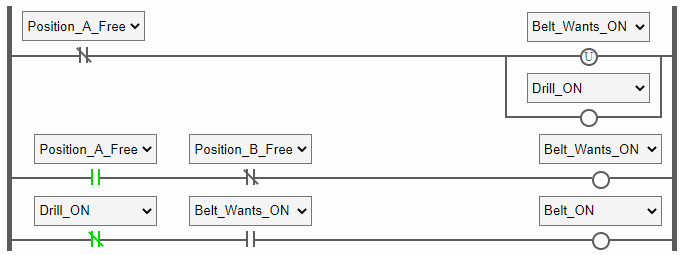
\includegraphics[width=\textwidth]{Figures/belt_drill_ld.png}
	\caption[Drill and Belt controller example in Ladder Diagram]{Drill and Belt controller example in Ladder Diagram}
	\label{fig:drill:ld}
\end{figure}
	%&tex
% !TEX program = xelatex
% !TeX TS-program = xelatex
% !BIB TS-program = biber
% !TeX encoding = UTF-8
% !TeX spellcheck = en_US
% !TeX root = ../thesis.tex
%% ==============================
\section{C-based Programming Methods}
\label{sec:c_methods}
%% ==============================

C is one of the most used programming languages of the last decades.
Its closeness to the actual hardware, the access to low level features, like memory management, and the low overhead make it the ideal system programming language.
Today big parts of operating systems, many embedded and real-time applications are written in C.
This makes it a prime candidate for~\acrshort{acn:plc} programming.
As its initial introduction was in the year 1972~\cite{10.5555/576122}, there are many libraries and frameworks available today, that are implemented in C.
The importance as a system programming language has also sparked intensive research in the field of formal verification of C code\todo{Add citation for formal C verification programs.}.

It is a standardized ISO language~\cite{ISO:9899:2018}, with the current C18 standard.
The most common and best supported C standard is the ANSI C / C90 standard from 1990.

The low overhead of C code allows the programmer to write programs that have a fairly deterministic runtime behavior.
This makes it one of the prime candidates for real-time systems.
On the other hand, its low level of abstraction makes writing more complex code, e.g for visualization, more complex and error prone that other high level languages.
But in order to efficiently and correctly program in C, a developer requires at least some experience in programming and concepts like pointer and memory management.
For this reason, C wasn't considered suitable for programming PLC's when they were initially developed.
Many automation engineers had a background electrical engineering rather than in computer science.
As PLC's were programmed by them, they developed languages that abstracted the problem to be closer to electrical and logical circuits.

Nowadays many people are proficient in programming, allowing the usage of C in automation tasks.
Therefore there are some~\acrshort{acn:plc} environments that allow for the developer to use C and C++ to program their~\acrshort{acn:plc}.
In this section I am going to the two major environments that allow for pure C/C++ programming on~\acrshort{acn:plc}.

\subsection{B \& R Automation Studio}

\todo[inline]{B \& R Automation Studio C/C++ Module Support}

\subsection{Beckhoff TwinCAT 3}

\todo[inline]{Beckhoff TwinCAT3 industrial PC C/C++ Runtime Modules}

	%&tex
% !TEX program = xelatex
% !TeX TS-program = xelatex
% !BIB TS-program = biber
% !TeX encoding = UTF-8
% !TeX spellcheck = en_US
% !TeX root = ../thesis.tex
%% ==============================
\chapter{Formal Specification-Based Methods}
\label{sec:formal_methods}
%% ==============================

Two of the most important aspects when programming a~\glspl{acn:plc} are validation and verification.
Validation describes the correctness of the specification compared to the intended use and verification is the correctness of the actual code compared to the specification.
Both of these aspects ensure that the system behaves as intended.
As~\glspl{acn:plc} are used for real-time applications, the importance of these factors increases even more.
The previously described methods for programming with C offered possibilities in that regard, but they did not improve significantly compared to the IEC 61131-3 languages.
Therefore in this section I am investigating the possibilities of using a formal specification to automatically program a PLC.
This allows to easier validate and verify the code that developed.
\citeauthor{Frey:2000aa}\todo{Formal methods in PLC programming} describe different approaches to verification and validation for~\acrshort{acn:plc} programming.
This paper also gives an overview of different methods that can be used to archive this.
From this overview I investigated the three most used techniques in the following section.

There a several methods for creating a formal specification of a process or controller.
One method is to use a formal language to specify the behavior in rules.
This method allows for easier verification and validation as the specification and code can checked via formal theorem solvers.
Approaches employing this method are described in subsection~\ref{sec:sub:flb}.

Another method is to use a modeling language to create a system specification.
A modeling language allows the user to create a structural and behavioral specification of the system.
This is in contrast to the formal languages that only describe behavioral details, but not structures.
They also allow for simulation of the system components making it easier to evaluate and validate the system.
In software development, model specifications like~\acrfull{acn:uml} are common practice.
The usage of a model can also provide a overview of the system and increase modularity.
In subsection~\ref{sec:sub:mb} I investigate approaches using this specification type.

The last approach I investigate are graph based specifications.
They are often used for behavioral descriptions in modeling languages but can also be used just to create a behavioral model.
They use system states and transitions between the states to model a event reaction semantic of the system.
Common approaches here are petri nets and condition graphs.
I describe these approaches in subsection~\ref{sec:sub:graph}.

\subsection{Formal Language Based}

\subsubsection{Linear Temporal Logic}

\todo[inline]{Construction and Verification of PLC Programs by LTL Specification}

\todo[inline]{Synthesizing Executable PLC Code for Robots from Scenario-Based GR(1) Specifications}

\subsubsection{PLCspecif}

\todo[inline]{PLC Code Generation Based on a Formal Specification Language}

\subsection{Model Based}

\subsubsection{UML / SysML}

\todo[inline]{Automated PLC Software Testing using adapted UML Sequence Diagrams}

\todo[inline]{A Model-Driven Approach on Object-Oriented PLC Programming for Manufacturing Systems with Regard to Usability}

\todo[inline]{Automatic Generation of Implementation in SysML-based Model-Driven Development for IEC 61131-3 Control Software}

\subsubsection{Simulink}

\todo[inline]{Model-based Verification of PLC programs using Simulink Design}

\todo[inline]{Comparison of a transformed Matlab/Simulink model into the programming language CFC on different IEC 61131-3 PLC environments}


\subsection{Graph Based}

\todo[inline]{Template-Based Generation of PLC Software from Plant Models Using Graph Representation}

	%&tex
% !TEX program = xelatex
% !TeX TS-program = xelatex
% !BIB TS-program = biber
% !TeX encoding = UTF-8
% !TeX spellcheck = en_US
% !TeX root = ../thesis.tex
%% ==============================
\section{Risks of Automated Programming}
\label{sec:risks}
%% ==============================

\subsection{Transformation Function Correctness}

\todo[inline]{Conversion of ST Control Programs to ANSI C for Verification Purposes}

\subsection{Validity of the Models}

\subsection{Runtime system guarantees}
	%&tex
% !TEX program = xelatex
% !TeX TS-program = xelatex
% !BIB TS-program = biber
% !TeX encoding = UTF-8
% !TeX spellcheck = en_US
% !TeX root = ../thesis.tex
%% ==============================
\chapter{\iflanguage{ngerman}{Zusammensaffung und Ausblick}{Conclusion}}
\label{sec:conclusion}
%% ==============================

In this seminar work I investigated multiple approaches on automated programming of~\acrlong{acn:plc}s.
First I presented two development environments that allow programming in higher level languages that the common IEC 61131-3 languages.

Secondly I looked at approaches to program~\acrshort{acn:plc}s from a high-level formal behavior description or a model of the process.
These approaches are compared on their effectiveness, efficiency, user-acceptance and real-world applicability.
All of the presented approaches provided good effectiveness for specifying the behavior on a higher abstraction level.
They excel at designing larger systems with complex behaviors and provide benefits compared to the traditional PLC programming methods, especially when looking at~\acrshort{acn:LD}.
With all of them allowing for formal verification of the defined behavior they are way less prone to faults introduced in the design and implementation phase of development.
When looking at efficiency, the plcSpecif, Simulink and modAT4rMS approaches allowed the developer to progress significantly faster with a lower probability of errors compared to traditional programming.
Methods, like the ones presented in~\ref{sec:sub:ltl}, on the other hand provided lower efficiency as their complex syntax makes development more time intensive.
The approaches that used pre-existing commonly used modeling notations, like UML, SysML or Simulink, benefited from a greatly improved user-acceptance.
They also required less additional training to be used in a effective manner.
Real-world usability is a more complex topic to address, as not all presented approaches aimed towards becoming a standard approach for programming~\acrshort{acn:plc}s.
Approaches like the GRAFCET,  plcSpecif and modAT4rMS based ones described development environments and implementations of the generation algorithms for real-world usage.
The~\acrshort{acn:ltl} based approaches on the other hand, aimed more towards a theoretical method.

As~\acrshort{acn:plc}s are commonly used in safety critical environments that required exact timing behavior to ensure safe operation.
Therefore the risk associated with automated programming are addressed.
Here I consider two major factors, the risk associated with the transformation from the model to the code and the risk associated with the runtime behavior of the system.
The transformation function has to ensure that the behavior of the design is correctly mapped to the code.
To ensure this, a approach has to give a extensive formulation of the transformation used.
All of the presented approaches provided, to some extend, a proof that their transformation function is correctly mapping the specification to the code.
Some approaches, like the plcSpecif or the modAT4rMS based approaches even provided extensive specification on the transformation, increasing the trustworthiness of their approach.
When looking at the runtime behavior, the automated programming introduces a lot of risk to the system.
The custom behavior of the models, that is mapped to the PLC cycles, makes it hard to give accurate predictions on the runtime behavior of the system.
In combination with the possible size of the generated model, this introduces large problems offsetting most of the development time advantages of automated programming methods.

In summary, there are a lot of methods for high-level and automated programming of~\acrlong{acn:plc}s.
They provide considerable advantages for designing large, complex system.
The available verification and validation methods make them less prone to faults in design and implementation.
But where they excel at efficiency and effectiveness during the design, they have significant disadvantages when looking at the deployment and the runtime guarantees that can be given.
They require in depth analysis on the deployment platform, offsetting a lot of the aforementioned advantages.
Still I think that automated programming for~\acrshort{acn:plc} is a promising topic of research and with improved development toolsets for the approaches, the disadvantages can be negated almost entirely.
	
	%% --------------------
	%% |   Bibliography   |
	%% --------------------
	%\nocite{*}
	\Bibliography
	
	%% ----------------
	%% |   Appendix   |
	%% ----------------
	\cleardoublepage
%	%% appendix.tex
%%

%% ==============================
\Appendix
%% ==============================

\dots
\section{First Appendix Section}
\label{sec:app-first-sections}



\begin{figure} [ht]
  \centering
   ein Bild
  \caption{A figure}
  \label{fig:BPMNBeispiela}
\end{figure}


\dots




	
	% Remove if needed
	%% -----------------------------
	%% |   List of Figures/Tables  |
	%% -----------------------------
	\includeglossaries
	\inculdelistoffigures
	\inculdelistoftables
	\inculdelistoflistings
	%\inculdelistofalgoritms
	
	%% --------------------
	%% |   MyBib Entry    |
	%% --------------------
	\addmybibentry
	
	%% --------------------------------
	%% |   How to use this document   |
	%% --------------------------------
	%\includehowtouse
	
\end{document}
